%# -*- coding: utf-8-unix -*-
% !TEX program = xelatex
% !TEX root = ../thesis.tex
% !TEX encoding = UTF-8 Unicode

\section{概述}%intro
\label{sec:compqa-intro}


基于知识库的自动问答(KBQA)是自然语言处理中的经典应用场景。
该任务以自然语言问句作为输入,
并根据已有结构化知识库提供的信息,寻找到问句的一个或多个答案。
以Freebase,YAGO,DBPedia为代表的结构化知识库
主要以维基百科为骨架构建而成,它们包含真实世界的广域知识,因此常用于自动问答任务中。

%The knowledge-based question answering (KBQA) is a task which 
%takes a natural language question as input and returns a factual answer 
%using structured knowledge bases
%%organizing open domain facts in the real world,
%such as Freebase~\cite{bollacker2008freebase},
%YAGO~\cite{suchanek2007yago} and DBpedia~\cite{auer2007dbpedia}.
%%organize massive open domain facts in the real world,
%%and make KBQA an open and popular research task,


在自动问答任务中,我们关注的问题称为``{事实类问题}'' ,其特点在于
它们询问的是与句子中实体相关的客观事实,因此答案为知识库中存在的实体、数值或时间。
以一个较简单的问题为例,``What's the capital of the United States?'' ,
为了准确回答这个问题,一个较为直接的方式是,首先识别句子中的相关实体并链接到知识库,
再将该实体与目标答案之间的自然语言关系映射为知识库中的一个谓词(或为词序列),
那么原问题即可转换为具有(实体,谓词,目标答案)三元组形式的查询语句,
例如($united\_states$, $capital$, $?$),通过在知识库上运行查询语句,生成最终的结果。
将已有的\textless 问题,答案 \textgreater 对作为训练数据,
我们可以通过远距离监督(Distant Supervision)的形式学习问句和查询语句之间的映射关系。

%%The questions in KBQA task are factual questions,
%%since the answer of each question is an object entity\footnote{Could be type or literal value}
%%of an existing subject entity in the question.
%One simple example is a question like this: ``What's the capital of the United States?''
%%we need to first recognize the subject named entity in the question,
%%for example, \textit{united\_states} in Freebase,
%%then understand the relation ``capital of'' connecting the subject and object answer,
%%is represented by the predicate \textit{location.location.capital} in FB, for example.
%A common answer to such question is to identify the focus entity
%and the main relation predicate (or a sequence) in the question, and 
%map the question to a triple fact query ($US$, $capital$, $?$) over KB.
%The object answers are returned by executing the query.
%The mapping above is typically learned from question-answer pairs
%through distant supervision.


对于只包含简单语义的问题,我们可以通过上述方法将其转为知识库上的一个基本三元组查询,
但这样的方法并不适用于其它具有更复杂语义的问题。
例如\figref{fig:compqa-intro}所示,为了准确回答问题
``What is the second longest river in United States?'' ,
我们实际上需要对其进行推理,得出以下三条语义线索:
1) 答案实体位于美国内部;
2) 答案实体的类型是河流;
3) 在满足前两个条件的所有实体中,根据长度属性进行降序排列,目标答案排在第二位。
具体分析,第一条语义类似于简单问题,描述相关实体和答案间的关联,
第二条语义则描述了知识库中的特定类型与答案的包含关系,
第三条语义和序数相关,它甚至不能简单地对应到知识库中已有的事实三元组。
由此可见,我们需要挖掘出多条不同的关系,才能准确地定位目标答案。
对于这类无法通过单个三元组查询来精确描述语义的问题,
我们将它称为``{复杂问题}'' ,也是这个章节研究的重点。

\begin{figure}[ht]
	\centering
    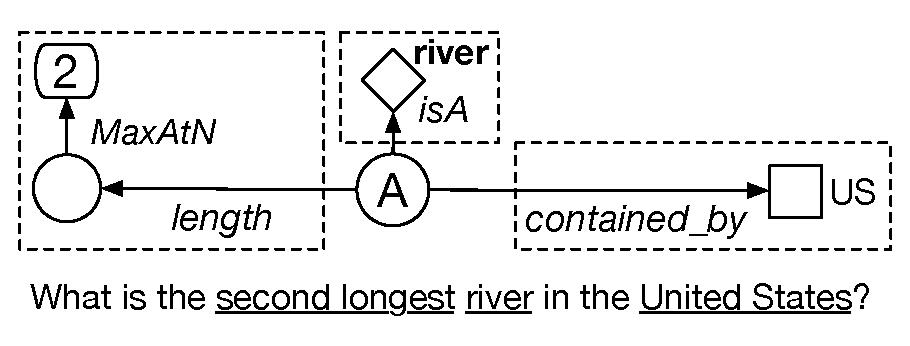
\includegraphics[width=0.7\columnwidth]{figure/compqa/intro.eps}
	%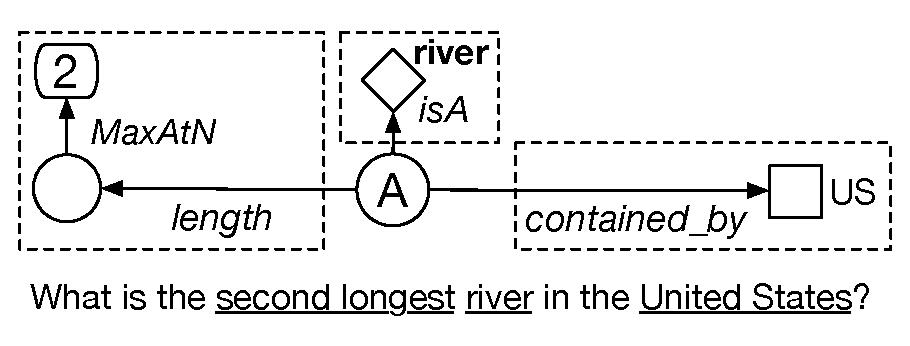
\epsfig{file=figure/compqa/intro.eps, angle=0, width=1.0\columnwidth}
	%\scalebox{0.3}{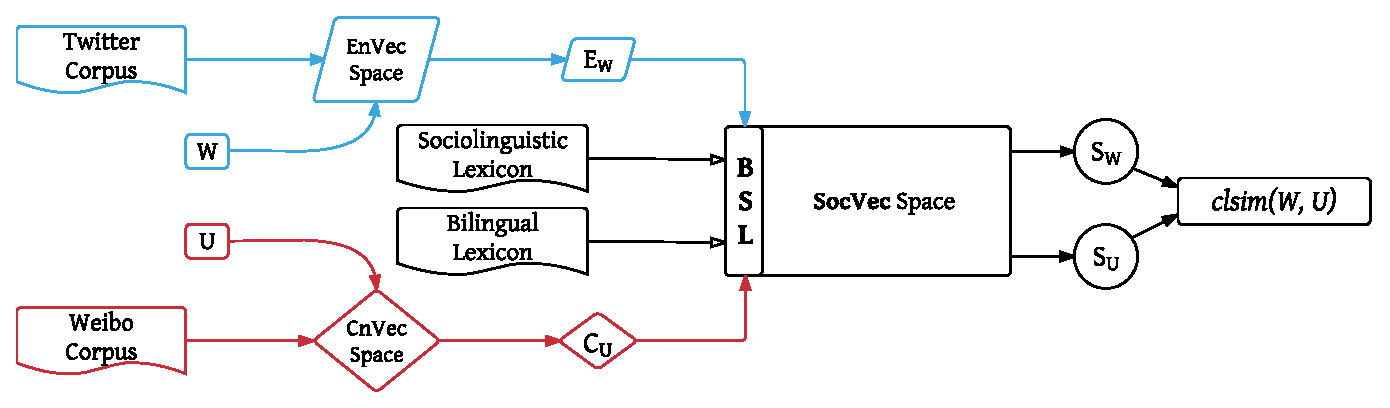
\includegraphics{overview.eps}}
	\bicaption{一个具有复杂语义的问句示例。}{Running example of complex question.}
	\label{fig:compqa-intro}
\end{figure}

%While the above question can be answered by querying
%a single predicate or predicate sequence in
%the KB, many other more complex questions cannot, e.g. the question
%in \figref{fig:intro}.
%%However, KBQA is not a trivial task,
%%because we are facing questions more complex than the previous case,
%%where the semantics of the question is not expressed by a single triple fact.
%%One question could have several focus entities,
%%like ``Who played Bilbo Baggins in the Hobbits'',
%%where both the character and the film are focus entities.
%%Our running example in \figref{fig:intro} is even more complex,
%To answer the question ``What is the second longest river in United States'',
%we need to infer several semantic clues:
%1) the answer is contained by United States;
%2) the answer is a river;
%3) the answer ranks second by its length in descending order.
%Thus, multiple predicates are required to constrain the answer set,
%and we call such questions ``complex questions'' throughout this paper.
%%According to statistics reported by Bao et al.~\shortcite{bao2016constraint},
%%15\% questions in WebQuestions~\cite{berant2013semantic}, which is a 
%%popular KBQA dataset, are complex.
%%and the ComplexQuestions dataset is designed for measuring the quality
%%of KBQA systems on the complex scenario, where all questions are complex.





回答复杂问题的核心,在于问答系统是否能准确理解问句中多部分语义之间的组合关系,
而不仅仅是通过搜索的方式得到答案。
这条思路对应了解决自动问答的语义解析技术(Semantic Parsing)
\cite{kwiatkowski2013scaling,berant2013semantic}。
对于一个问句,基于语义解析的模型会将其转换成一棵语义解析树,
%CCG:自底向上将句子中的单词组合起来,语法以及语义:基于lambda表达式,
%有些词语充当function,有些则充当argument
%通过预定义的语法,自底向上形成整个树
%将pred和entity都映射到KB,
这样的解析树等价于知识库中的查询图(Query Graph),
与关系理解中的模式图类似,是包含未知实体知识库子结构。
本章中,``{语义解析树}'' , ``{查询结构}'' 和 ``{查询图}'' 表示同一概念。
\figref{fig:compqa-intro}为问题
``What is the second longest river in United States ?'' 的查询图,具有树形结构。
代表未知答案的节点A为解析树的根节点,
三个叶节点$US$,$river$,$2$则由问句的字面描述中抽取出来,
并已链接到知识库中的实体、类型、时间或是数值上。
这些叶节点通过知识库中的谓词(序列)与答案节点连接,
从而对未知答案进行限制,因此本节中也称叶节点为问句的``{相关节点}'' 。
此外,近年来神经网络模型在提高自动问答系统的性能方面显示出了巨大的前景,
在多个不同的自动问答数据集上,通过神经网络改善语义解析的方法成为了目前最先进的技术
\cite{yih2015semantic,bao2016constraint,xu2016question}。
基于以上论述,本章所讨论的工作围绕语义解析技术结合神经网络模型的思路,
并将其扩展至复杂问题场景。

%For answering complex questions, it's more important to understand the compositional
%semantic meanings of the question.
%%rather than directly outputting answer entities.
%As a classic branch of KBQA solutions, semantic parsing (SP) technique
%%Therefore, our research work is based on the semantic parsing (SP) technique
%~\cite{berant2013semantic,yih2015semantic,reddy2016transforming,hu2018answering}
%aims at learning semantic parse trees or equivalent query graphs
%\footnote{The term ``query graph'' is interchangeable
%with ``query structure'' and ``semantic parsing tree'' throughout this paper.}
%for representing semantic structures of the questions.
%For example in \figref{fig:intro}, the query graph forms a tree shape,
%where the focus nodes (\textit{US}, \textit{river}, \textit{2nd})
%are extracted from the mentions of the question,
%and the answer node is connected to these nodes via predicate 
%sequences in the knowledge base.
%%SP-based approaches first generate candidate graphs using
%%bottom up parsing~\cite{berant2013semantic,cai2013large}
%%or staged query generation methods~\cite{yih2015semantic,bao2016constraint}, 
%%then predict the best graph by calcuating the semantic similarity of the question.
%%Final answers are produced by executing the SPARQL query (shown in \figref{fig:intro})
%%translated from the query graph.
%Recently, neural network (NN) models have shown great promise in
%improving the performance of KBQA systems,
%and SP+NN techniques become the state-of-the-art on several KBQA datasets
%~\cite{qu2018question,bao2016constraint}.
%According to the discussion above, 
%our works extends the current research in the SP+NN direction.




%%4. challenge: candgen
%\KZ{Simplify these two challenges significantly.}
%We face two key challenges for answering complex questions.
%First, there is a large searching space to collect candidate query structures.
%For simple questions, the query structure is limited to 
%a single predicate connecting the focus entity and the answer.
%However, as illustrated in \figref{xxx},
%the query structure of a complex question has a tree shape with multiple edges,
%we can generate different candidates exponentially larger than
%the size we generated from simple questions.
%%4-1. other works
%Traditional semantic parsing approaches partially tackle the problem by
%introducing a ``bridge'' operation to merge simple facts into tree structure
%~\cite{berant2013semantic},
%or predefine a number of parsing templates with branches~\cite{bast2015more},
%Candidate structures can be translated from dependency parsing of the question~\cite{reddy2016},
%but it's highly relies on the parsing accuracy,
%and the translation rules need much human prior knowledge.
%There are approaches to circumvent the problem of candidate generation.
%For example, 
%Xu et al.~\shortcite{xu2016question} generated candidates in the form of single fact,
%and leverage unstructured text information to verify whethe a candidate answer
%satisfies other semantic constarints in the question.
%This approach is out of our discussion,
%as it can be regarded as a post-process step in the majority of KBQA frameworks.
%%4-2. yih & bao
%Recently, stagged query structure generation is a technique proved to be effective
%in research works~\cite{yih2015semantic,bao2016constraint}.
%The intuition is to generate query structure in step-by-step extension:
%starting from a focus entity extracted from the question, then explore candidate paths
%to the answer entity, and attach constraint paths in a depth-first search manner.
%
%Staged generation is proved to be effective and used in xxx research works.
%The difference: rules applied for particular constraints.
%
%%yih proposed a staged candidate generation scheme.
%%Based on candidate entities, search from one entity, and add constraints to the tree from other entity.
%%Bao is similar framework, considers entity / type / time / ordinal constraints with few handcrafted rules.
%%stage generation proves to be effective





语义解析模型可以分为两个部分:生成候选查询图,以及预测最佳查询图。
候选查询图的生成可以采用自底向上的方式构建\cite{berant2013semantic,berant2014semantic},
或是分阶段形式,由简到繁逐步生成所有候选\cite{yih2015semantic,bao2016constraint}。
预测最佳查询图,主要是基于计算问题和查询图之间的语义相似度,挑选出最佳查询图。
对于回答简单问题,目前已有的神经网络模型主要遵循 ``{编码-比较}'' 框架,
即首先利用卷积神经网络(CNN)或循环神经网络(RNN),
将原始问题以及候选的谓词序列分别进行编码,形成在同一个向量空间中的两个不同的语义向量,
两者之间的语义相似度则可以定义为向量空间中的距离度量。

当输入的问题具有复杂语义时,候选的查询图无法简化为线性的谓词序列,
如何对复杂的查询图进行编码,成为了语义相似度模型的关键问题。
一个较为直观的做法,是将整个查询图看做由答案节点到不同叶节点的路径集合,
%一个直观的做法,就是将整个查询图拆分为多个部分,%(换个词?)
例如\figref{fig:compqa-intro}中的虚线框将查询图分成三个语义成分,
分别对应指向不同相关实体的谓词序列。
%每个部分仅关心答案节点到一个叶节点的路径,即谓语序列,
%代表一部分的语义
这使得针对简单问题的神经网络模型可以被直接应用,
即分别计算问句与不同语义成分的相似度分值,并将其聚合(平均或相加),
用来代表问句与查询图整体的语义相似度。

这种基于查询图拆分的方式具有其合理性,
每个语义成分仅对应一个相关实体,类似人类对问句推理得到的平行语义线索。
然而,基于此法套用简单问题的神经网络模型,依然存在两个缺陷。
%每条谓语路径可以准确表示问句的部分语义
%有意义 但是优缺点
%这样的做法依然面临两个局限。
第一个缺陷是,将独立的语义成分与问句直接比较会带来风险。
对于简单问题,唯一的谓词路径代表了整个问句的语义,
%在信息量对等的情况下,
问句和查询对应的语义向量越相近,代表它们匹配度也越高。
然而复杂问题的查询图中,每一个独立的路径仅包含问句部分语义,
即便是正确的谓词路径,与问句整体依然存在语义差距。
%准确的来说,这是蕴含问题
若整体相似度由各部分相似度相加产生,则可能导致训练陷入局部极值,
%在没有海量训练数据的情况下,可能导致训练陷入局部极值。
即问句经编码后的语义向量倾向于查询图中的某条特定谓词路径,
而难以和其余正确的语义成分产生匹配。
%相加,有可能倾向于某些特定的路径,而认为其它路径并不正确。
第二个缺陷是,分别计算相似度再简单相加的形式会丢失信息。%(什么样的信息?)
将查询图的多个谓词序列分别进行编码,计算相似度再合并,
这样的做法视作互相独立的多个部分。
因此这样的模型无法理解不同语义成分之间存在的重叠、互补等语义交互。
模型没有学习整个查询图的语义向量,
%模型中没有向量对应整个查询图的语义表示,
因此无法从一个全局的角度描绘复杂查询图所包含的语义组合。

已有的文献\parencite{yih2015semantic,xu2016question}尝试规避上述两个缺陷,
它们的共同点在于从查询结构中仅挑选一条主路径,
与问句计算语义相似度,对于查询结构中的其它限制,
则依赖于人工定义的规则特征,或引入外部非结构化文本进行额外过滤。
问答模型效果得以提升,但并没有直接应对这样的不足。

在本章中,我们着手于利用神经网络模型改善问句与复杂查询图之间语义相似度计算的效果,
并尝试解决之前论述的两个缺陷。
该模型整体基于对问句和谓词序列的编码,将其表示为同一个语义空间下的语义向量。
我们的模型和之前方法主要区别,在于模型对各个语义成分编码后的向量进行结合,
形成对于查询图整体的语义向量表示。
同时,为了弥补问句和语义成分之间的信息不对等,在对问句进行编码的过程中,
我们利用依存语法分析(Dependency Parsing)寻找问句中和特定谓词序列相关的局部信号,
以此作为对问句字面信息的补充,使模型能更好地将问句和不同的语义成分对齐。
%TODO: ensemble和candgen要不在这里也说一下?

%%1. propose
%In order to attack the above limitations, we propose a neural network based 
%%approach to improve relation matching performance of complex question answering.
%approach to improve the performance of semantic similarity measurement
%in complex question answering.
%%\KZ{This is the first time u mention relation matching. Do they understand
%%what it is?}
%%2. basic
%Given candidate query graphs generated from one question,
%our model embeds the question surface and predicate sequences into a uniform 
%vector space.
%%3. combination
%The main difference between our approach and previous methods is that
%we integrate hidden vectors of various semantic components
%and encode their interaction as the hidden semantics of the entire query graph.
%%so that the model  encodes the semantics of whole graph structure.
%%4. dependency
%In addition, to cope with different semantic components of a query graph,
%we leverage dependency parsing information as a complementary of 
%sentential information for question encoding,
%which makes the model better align each component to the question.
%%5. eval
%%the module is able to handle both complex questions and simple questions.
%The contribution of this paper is summarized below.






本章的贡献可以总结为以下四个部分:
\begin{enumerate}
\item{提出了一个轻量化和有效的神经网络模型来解决具有复杂语义的自动问答任务。
据我们所知,这是第一次尝试在模型中对复杂查询图的完整语义进行明确编码;}
\item{通过融入依存语法分析信息来丰富模型中问句的语义表示,
并进行模型分析以验证其有效性;}
\item{通过一种集成的方法,对已有的实体链接工具进行改良,
丰富从问句中获得的候选实体,并进一步提升任务的整体效果;}
\item{在多个自动问答数据集上进行实验,在由复杂问题组成的ComplexQuestions数据集中,
模型的效果超过了已有的方法,在主要有简单问题组成的WebQuestions和SimpleQuestions数据集中,
模型依然具有很强的竞争力。}
\end{enumerate}

% candgen: less rules???? must be kidding me.
% model in general: interactive composing semantic components.
% model in detail: path embedding, rather than predicate word embedding?? (make use of ids and names)
% footnote: http://anonymous.for.double.blind.review

%\begin{itemize}
%\item We propose a light-weighted and effective neural network model to solve complex KBQA task.
%      To the best of our knowledge, this is the first attempt to
%      explicitly encode the complete semantics of a complex 
% 	  query graph (\secref{sec:rm});
%\item We leverage dependency parsing to enrich question representation 
%	  in the NN model, and conduct thorough investigations to 
%	  verify its effectiveness (\secref{sec:qw-repr});
%\item We propose an ensemble method to enrich entity linking from
%      a state-of-the-art linking tool, which further improves the 
%      performance of the overall task (\secref{sec:ensemble});
%
%\item We perform comprehensive experiments on multiple QA datasets,
%      and our proposed method consistently outperforms previous approaches 
%	  on complex questions, and produces competitive results on 
%	  datasets made up of simple questions (\secref{sec:exp}).
%\end{itemize}

%1. compact v.s. separated features (composition is better than isolated calculation) (interaction) (YES INTERATCTION, HOW to state?)
%   a. traditional: yih, xu, jain: ignore or postprocess
%   b. bao: simply weighted sum
%2. "context pattern" or other clues needed to send to the other side of BiCNN (ad-hoc to determine context pattern, not clearly mentioned)
%3. no need pre-train CNN (don't think pre-train is a good choice)

%Main part in the intro:
%  how to tackle the question with multiple constraints.
%  Imitate intro from Yih, Bao, Xu, Jain, Yin(f)...
%
%Interact:
%  semantic interact: (max pooling) simple but effective
%  entity linking: interactive feature (however, not used right now)
%
%RM helped by EL: raw score as evidence
%EL helped by RM: rare (RM is more reliable)
